Nuestro programa acepta una lista de largos de los histogramas en los que el histograma horiginal será separado.
Esta es la constante global \texttt{LARGOS} que puede encontrarse en \texttt{main.py}

Por ejemplo, si la lista es \texttt{[1, 2, 1, 1]}, significa que el histograma original será dividido en 4,
y que el segundo histograma de la separación medirá el doble que el resto.
Para dividir el histograma original en $n$ histogramas iguales basta con asignarle \texttt{[1 for \_ in range(n)]}
a la lista.

Como se observarán en los ejemplos que siguen, cambiar los intervalos de separación obviamente afecta
al histograma de salida, pero visualmente los cambios serán casi imperceptibles.

\subsection{Ejemplo 1}
Usamos la imagen \texttt{1906bxx}, con parámetros $\alpha = 0.1$, $\beta = 0.9$, $\gamma = 0.0$.

\begin{figure}[H]
\begin{minipage}[c]{0.48\linewidth}
  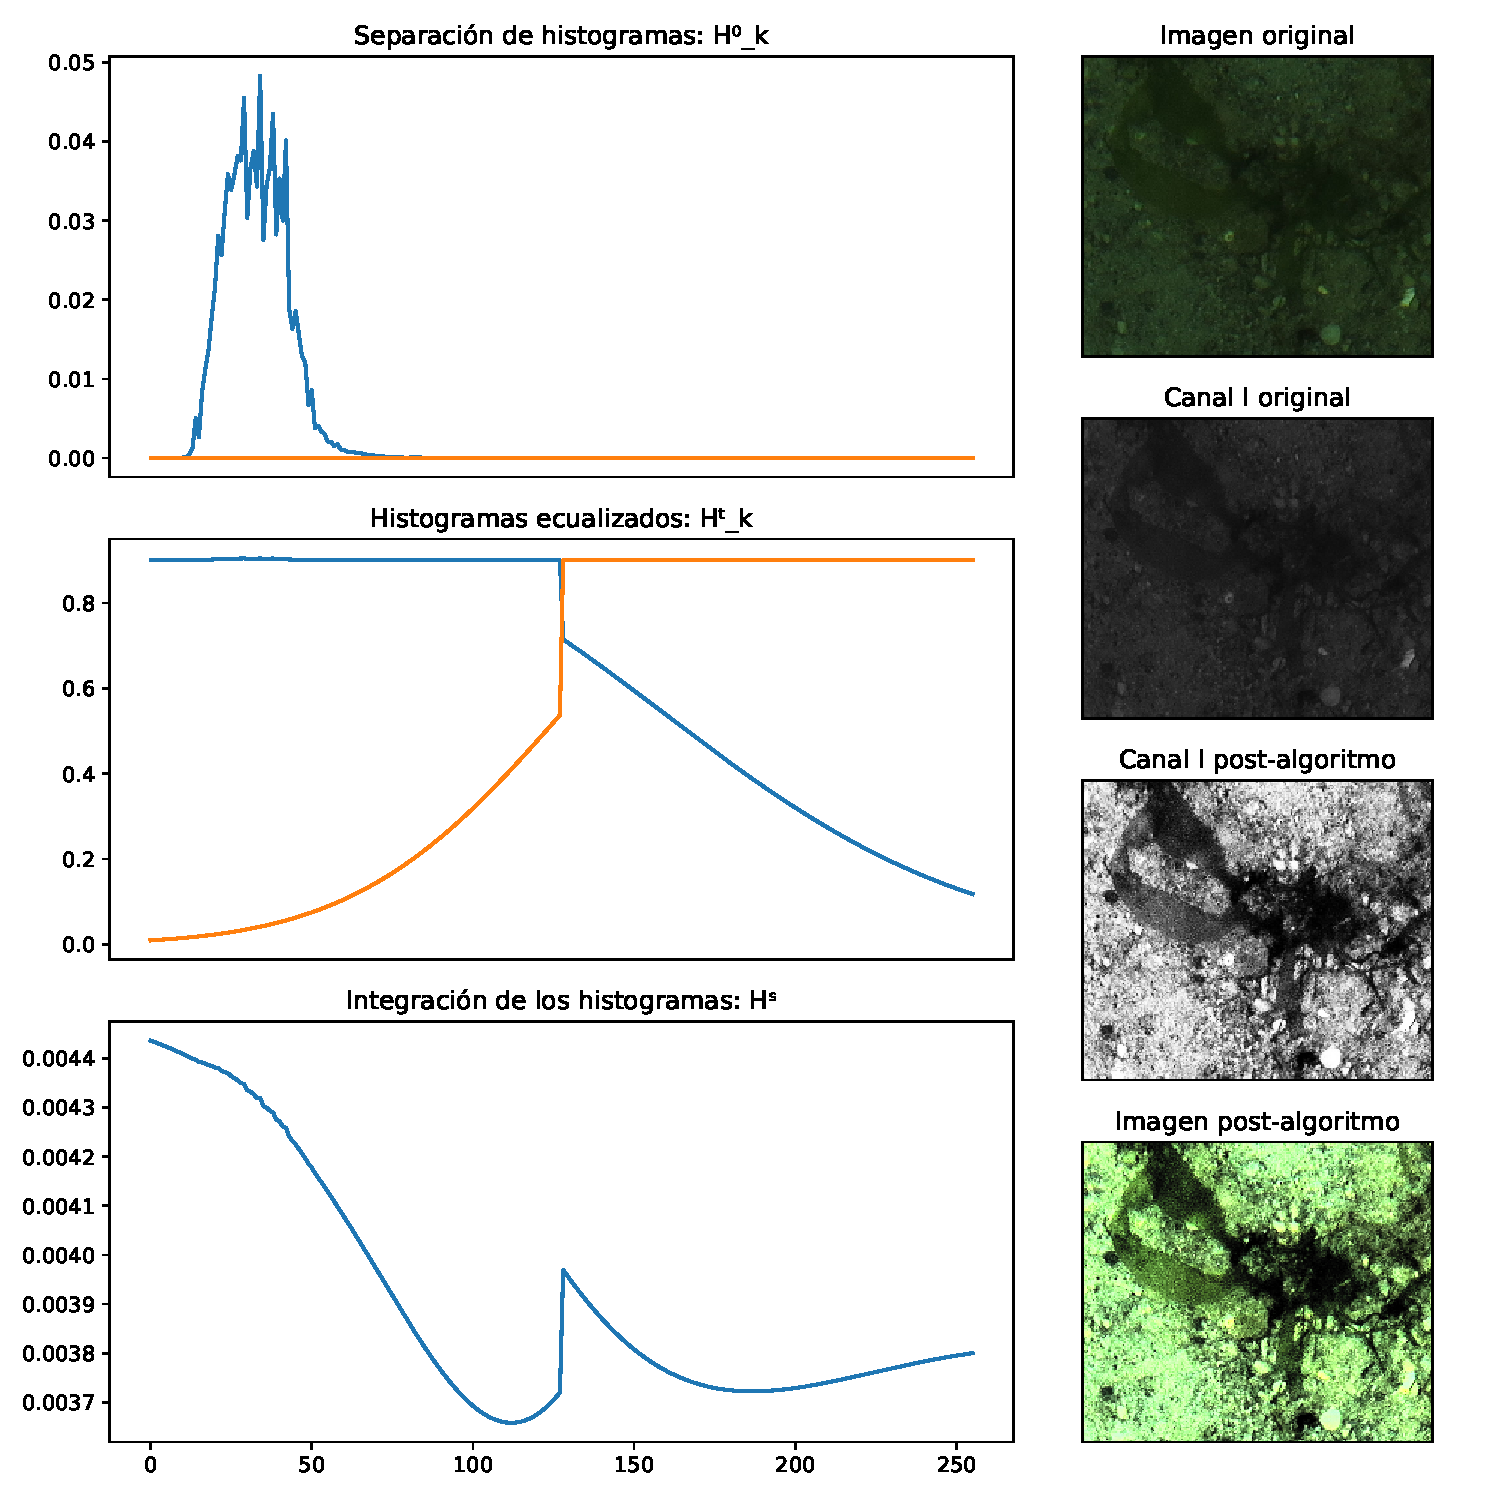
\includegraphics[height=9cm]{imgs/1906bxx-11.pdf}
  \caption{\texttt{[1, 1]}}
\end{minipage}
\hfill
\begin{minipage}[c]{0.48\linewidth}
  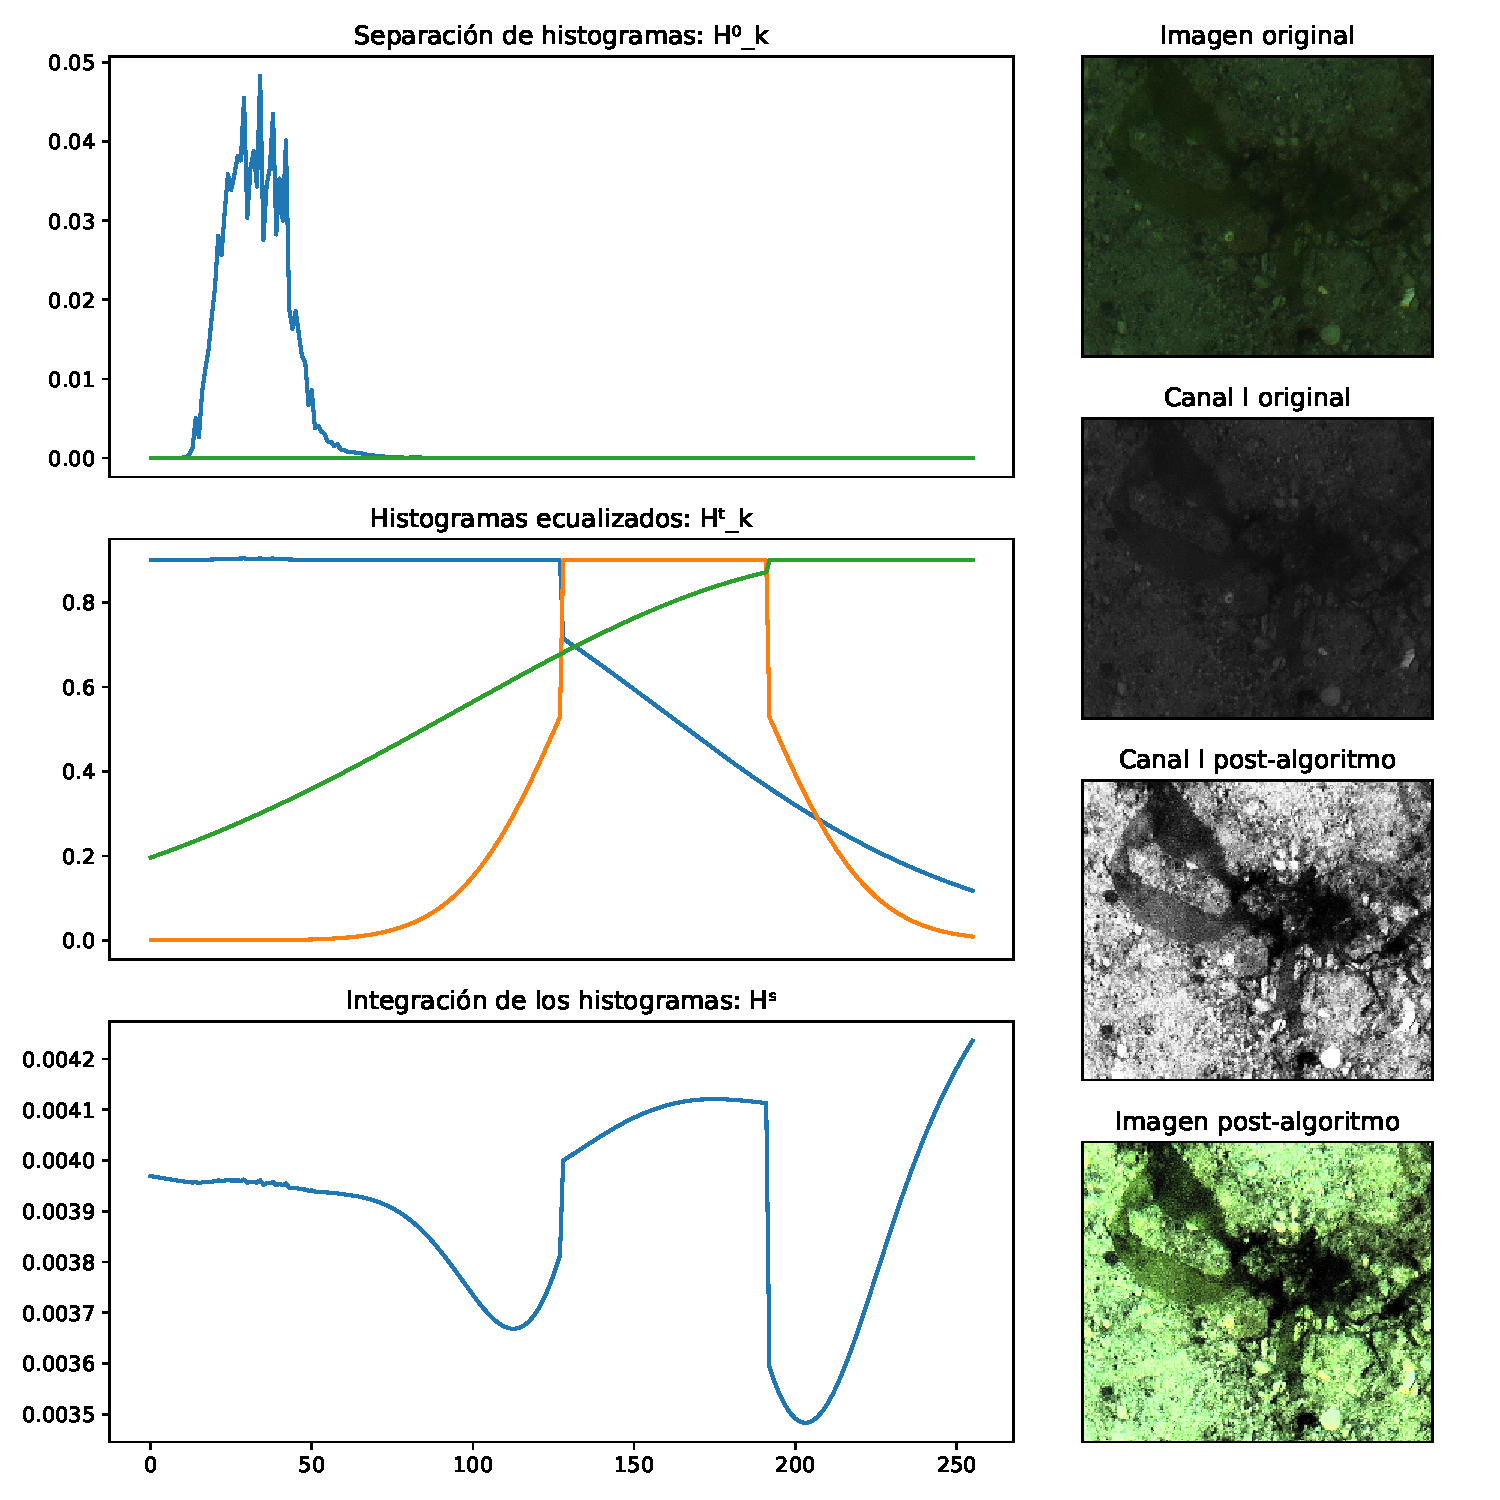
\includegraphics[height=9cm]{imgs/1906bxx-211.pdf}
  \caption{\texttt{[2, 1, 1]}}
\end{minipage}%
\end{figure}

i\begin{figure}[H]
\begin{minipage}[c]{0.48\linewidth}
  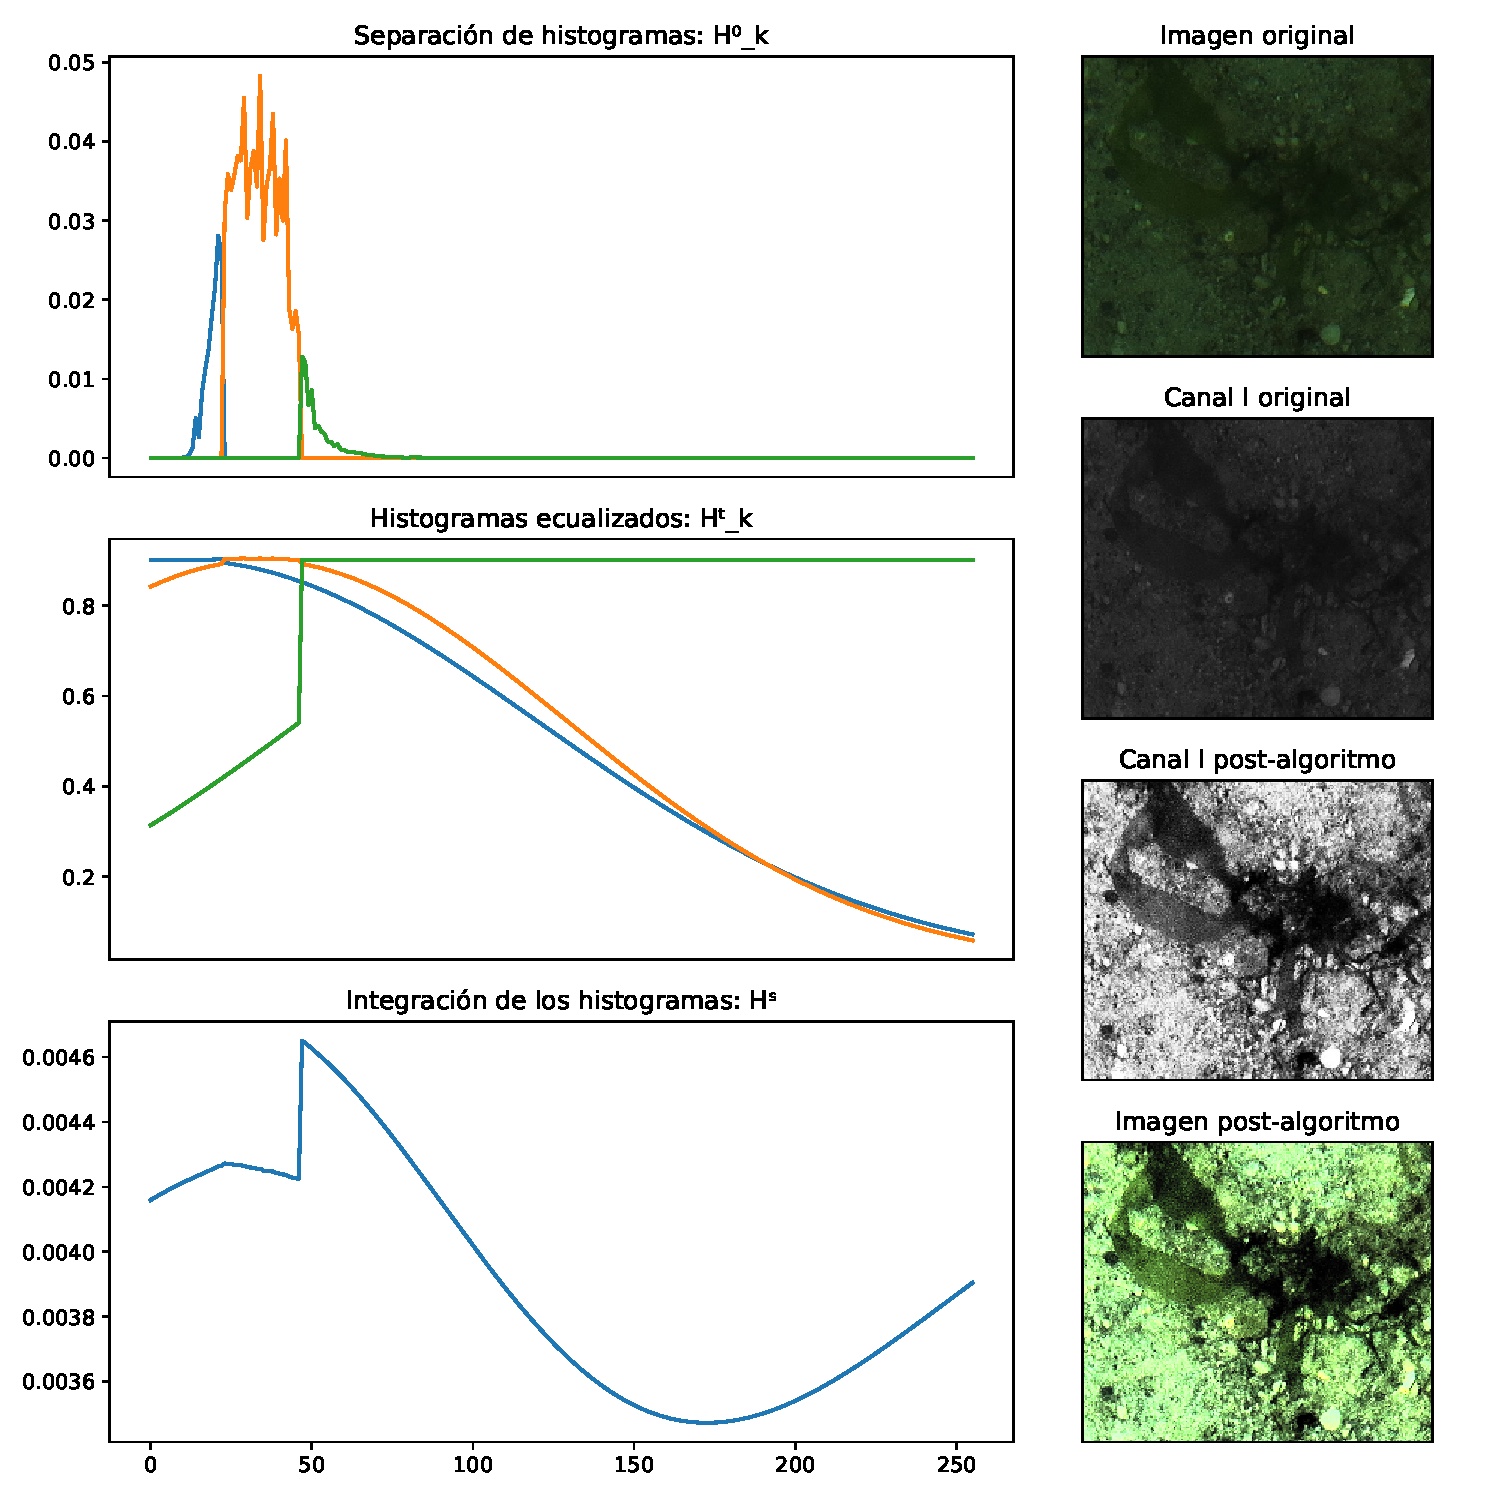
\includegraphics[height=9cm]{imgs/1906bxx-119.pdf}
  \caption{\texttt{[1, 1, 9]}}
\end{minipage}
\hfill
\begin{minipage}[c]{0.48\linewidth}
  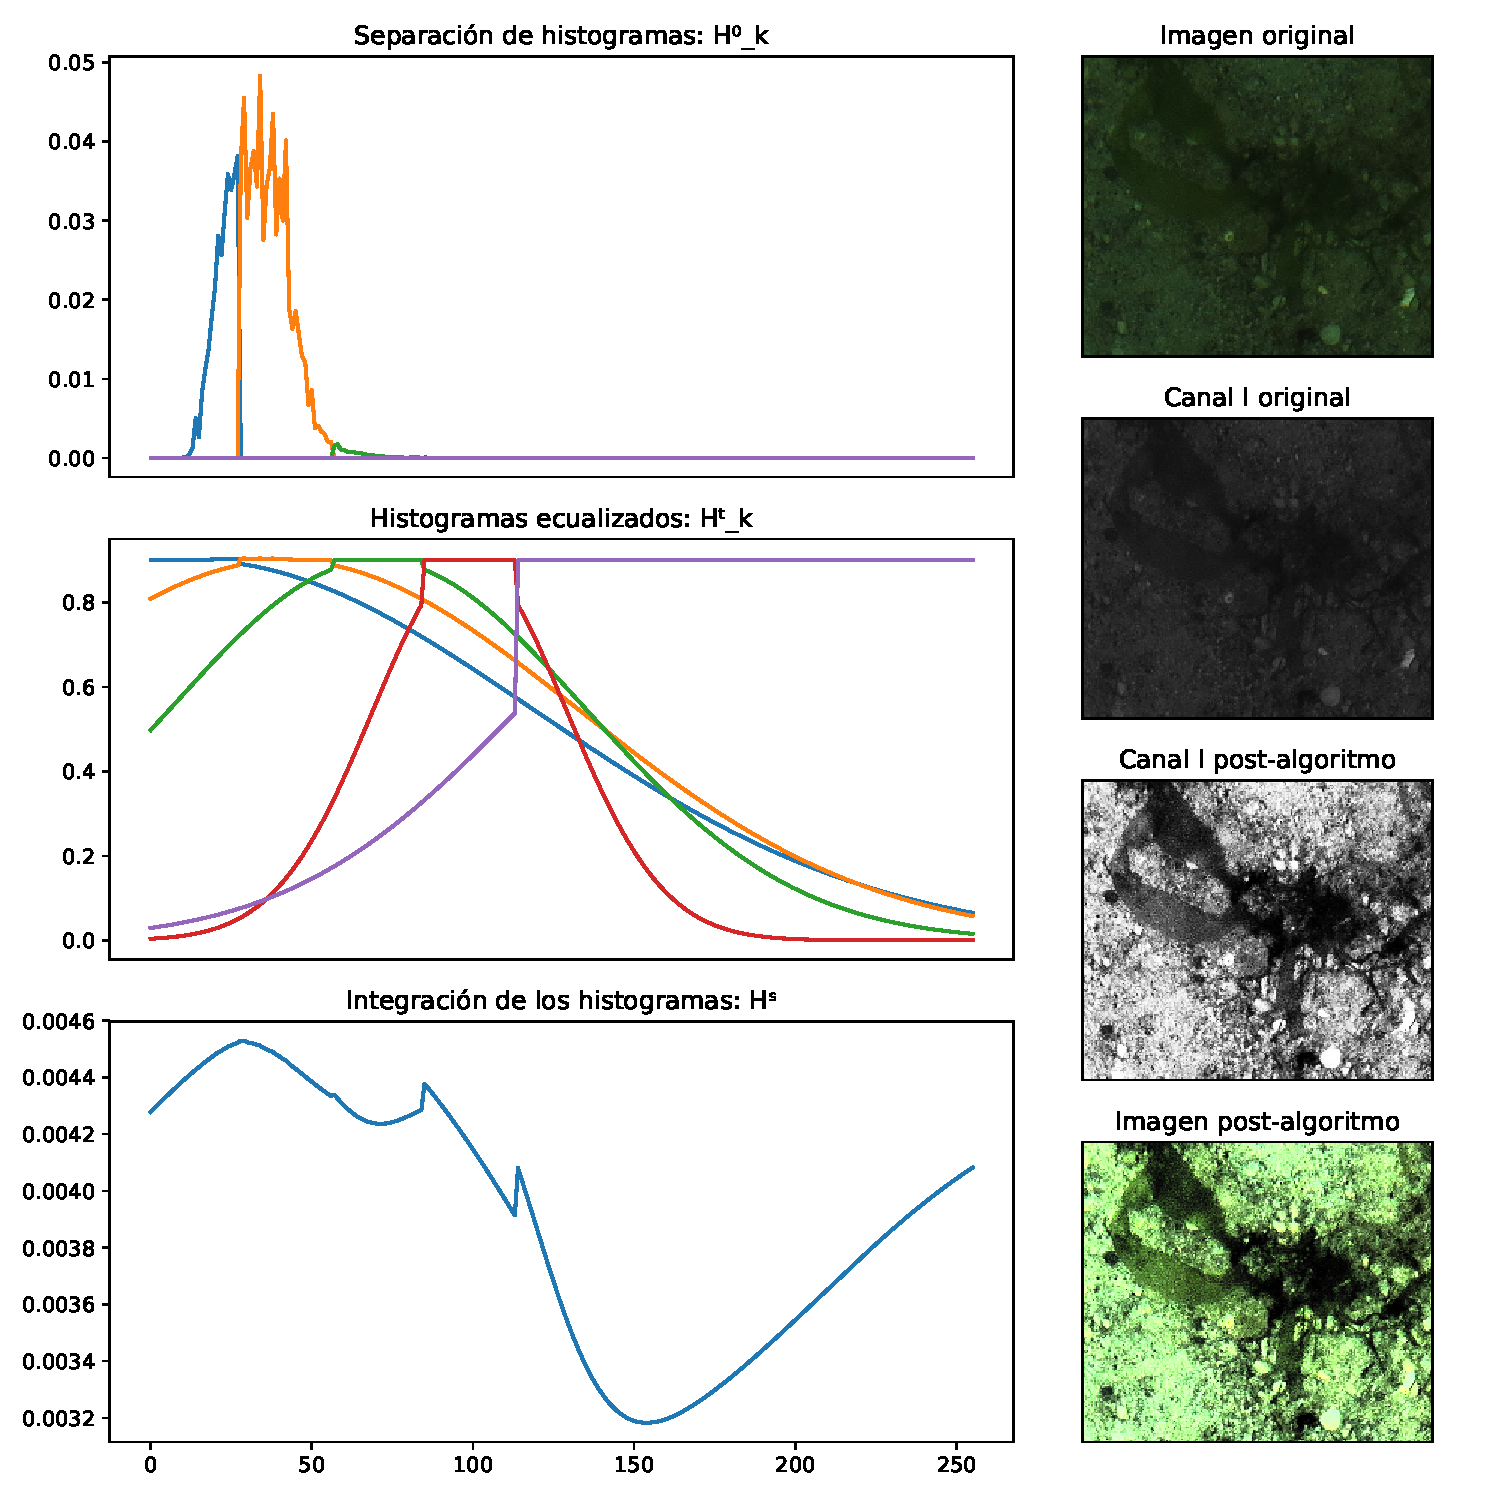
\includegraphics[height=9cm]{imgs/1906bxx-11115.pdf}
  \caption{\texttt{[1, 1, 1, 1, 5]}}
\end{minipage}%
\end{figure}

\subsection{Ejemplo 2}
Usamos la imagen \texttt{1906bxx}, con parámetros $\alpha = 0.8$, $\beta = 0.1$, $\gamma = 0.1$.

\begin{figure}[H]
\begin{minipage}[c]{0.48\linewidth}
  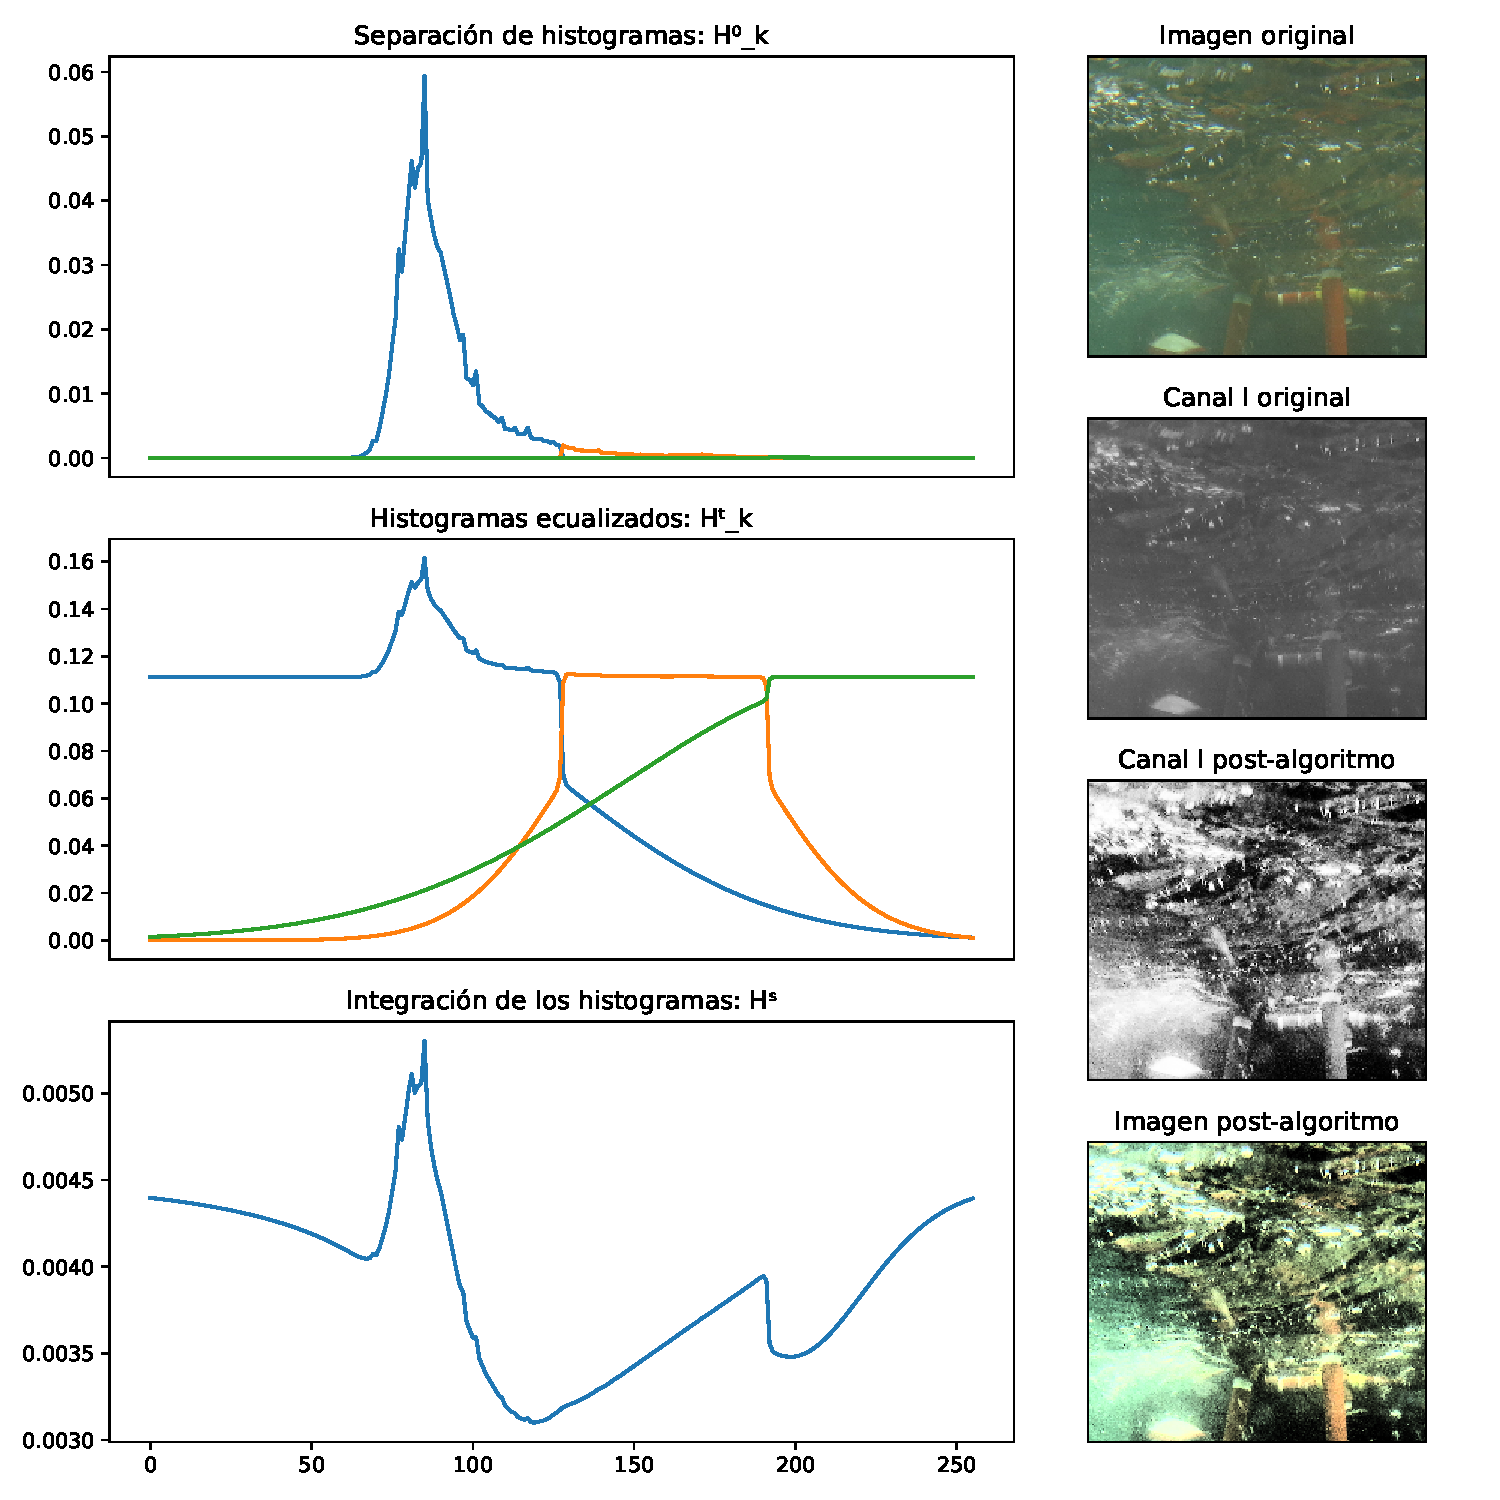
\includegraphics[height=9cm]{imgs/1908iv-211.pdf}
  \caption{\texttt{[2, 1, 1]}}
\end{minipage}
\hfill
\begin{minipage}[c]{0.48\linewidth}
  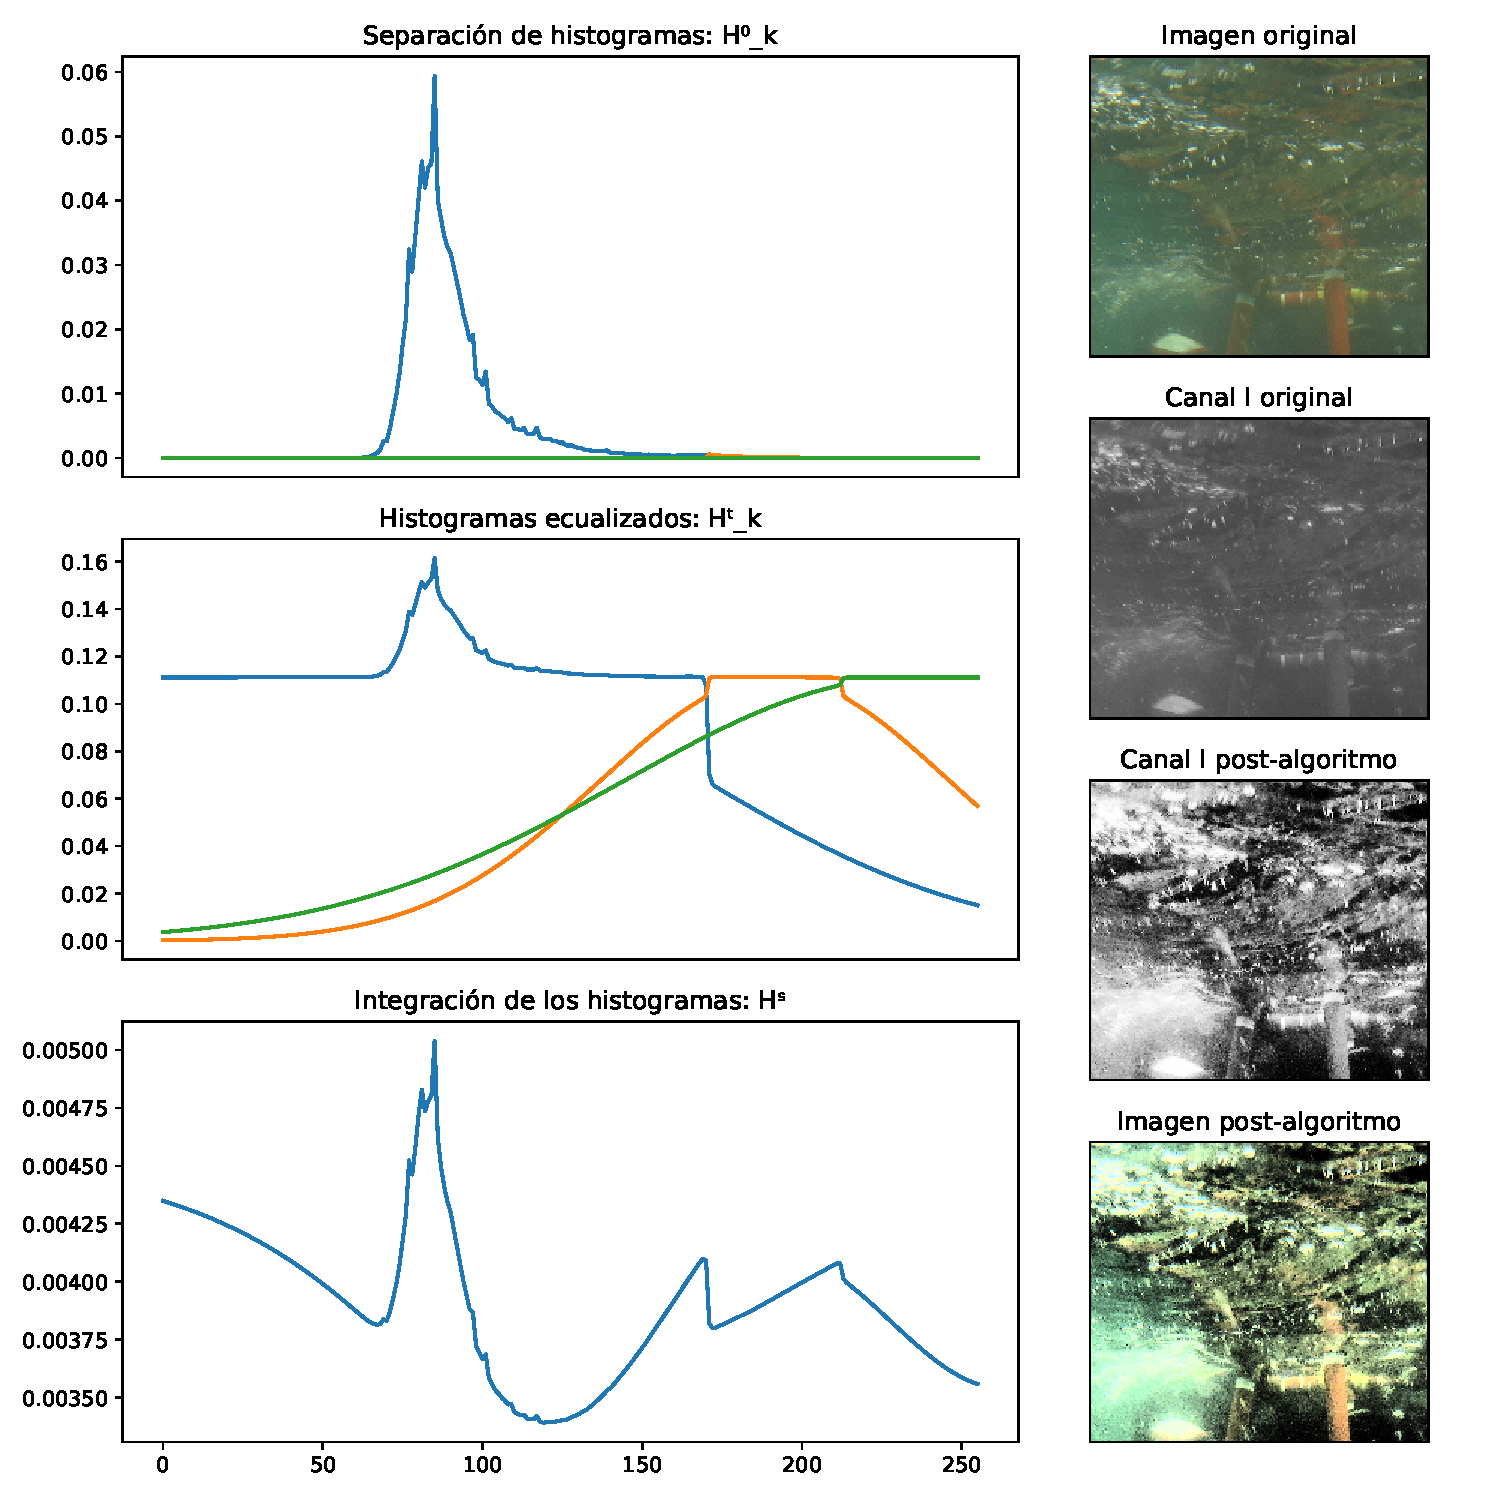
\includegraphics[height=9cm]{imgs/1908iv-411.pdf}
  \caption{\texttt{[4, 1, 1]}}
\end{minipage}%
\end{figure}

i\begin{figure}[H]
\begin{minipage}[c]{0.48\linewidth}
  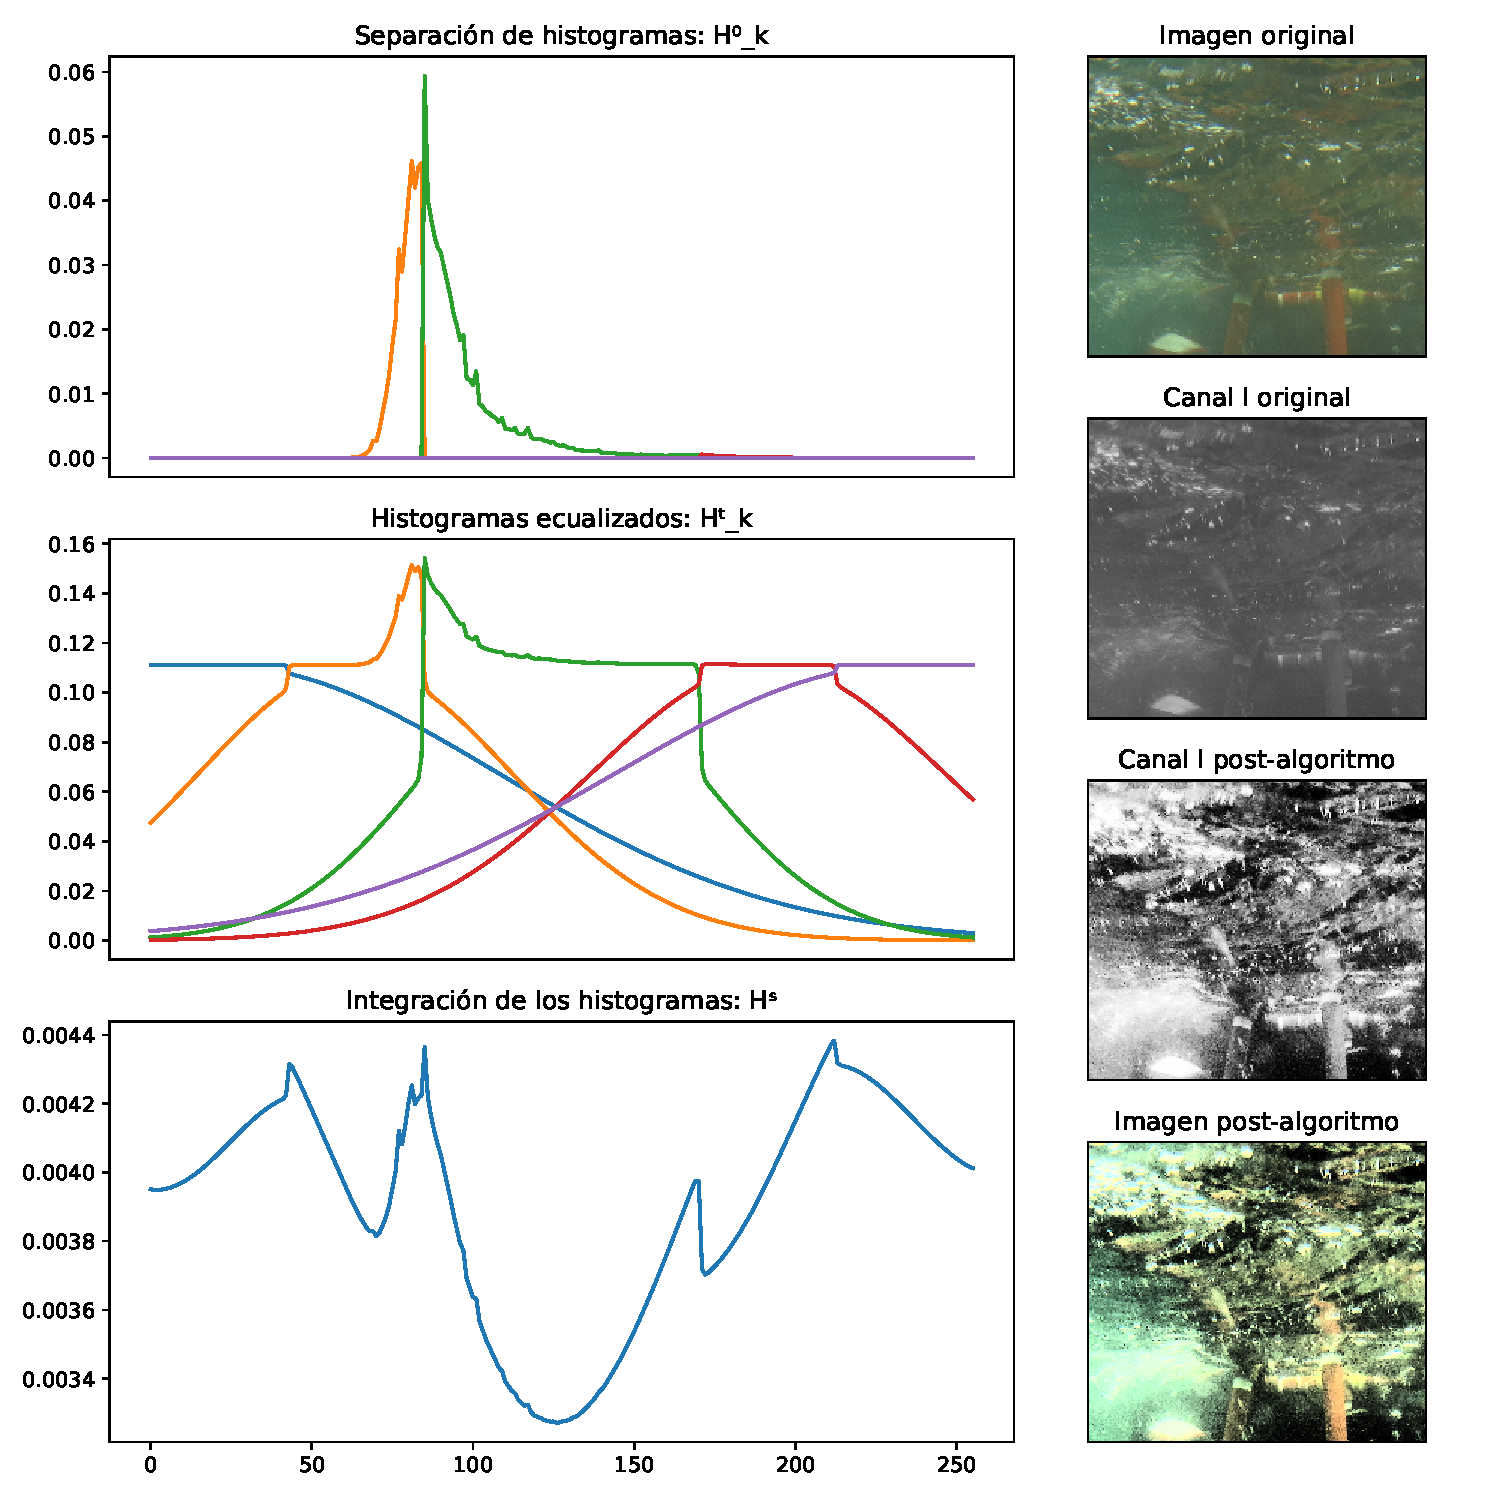
\includegraphics[height=9cm]{imgs/1908iv-11211.pdf}
  \caption{\texttt{[1, 1, 2, 1, 1]}}
\end{minipage}
\hfill
\begin{minipage}[c]{0.48\linewidth}
  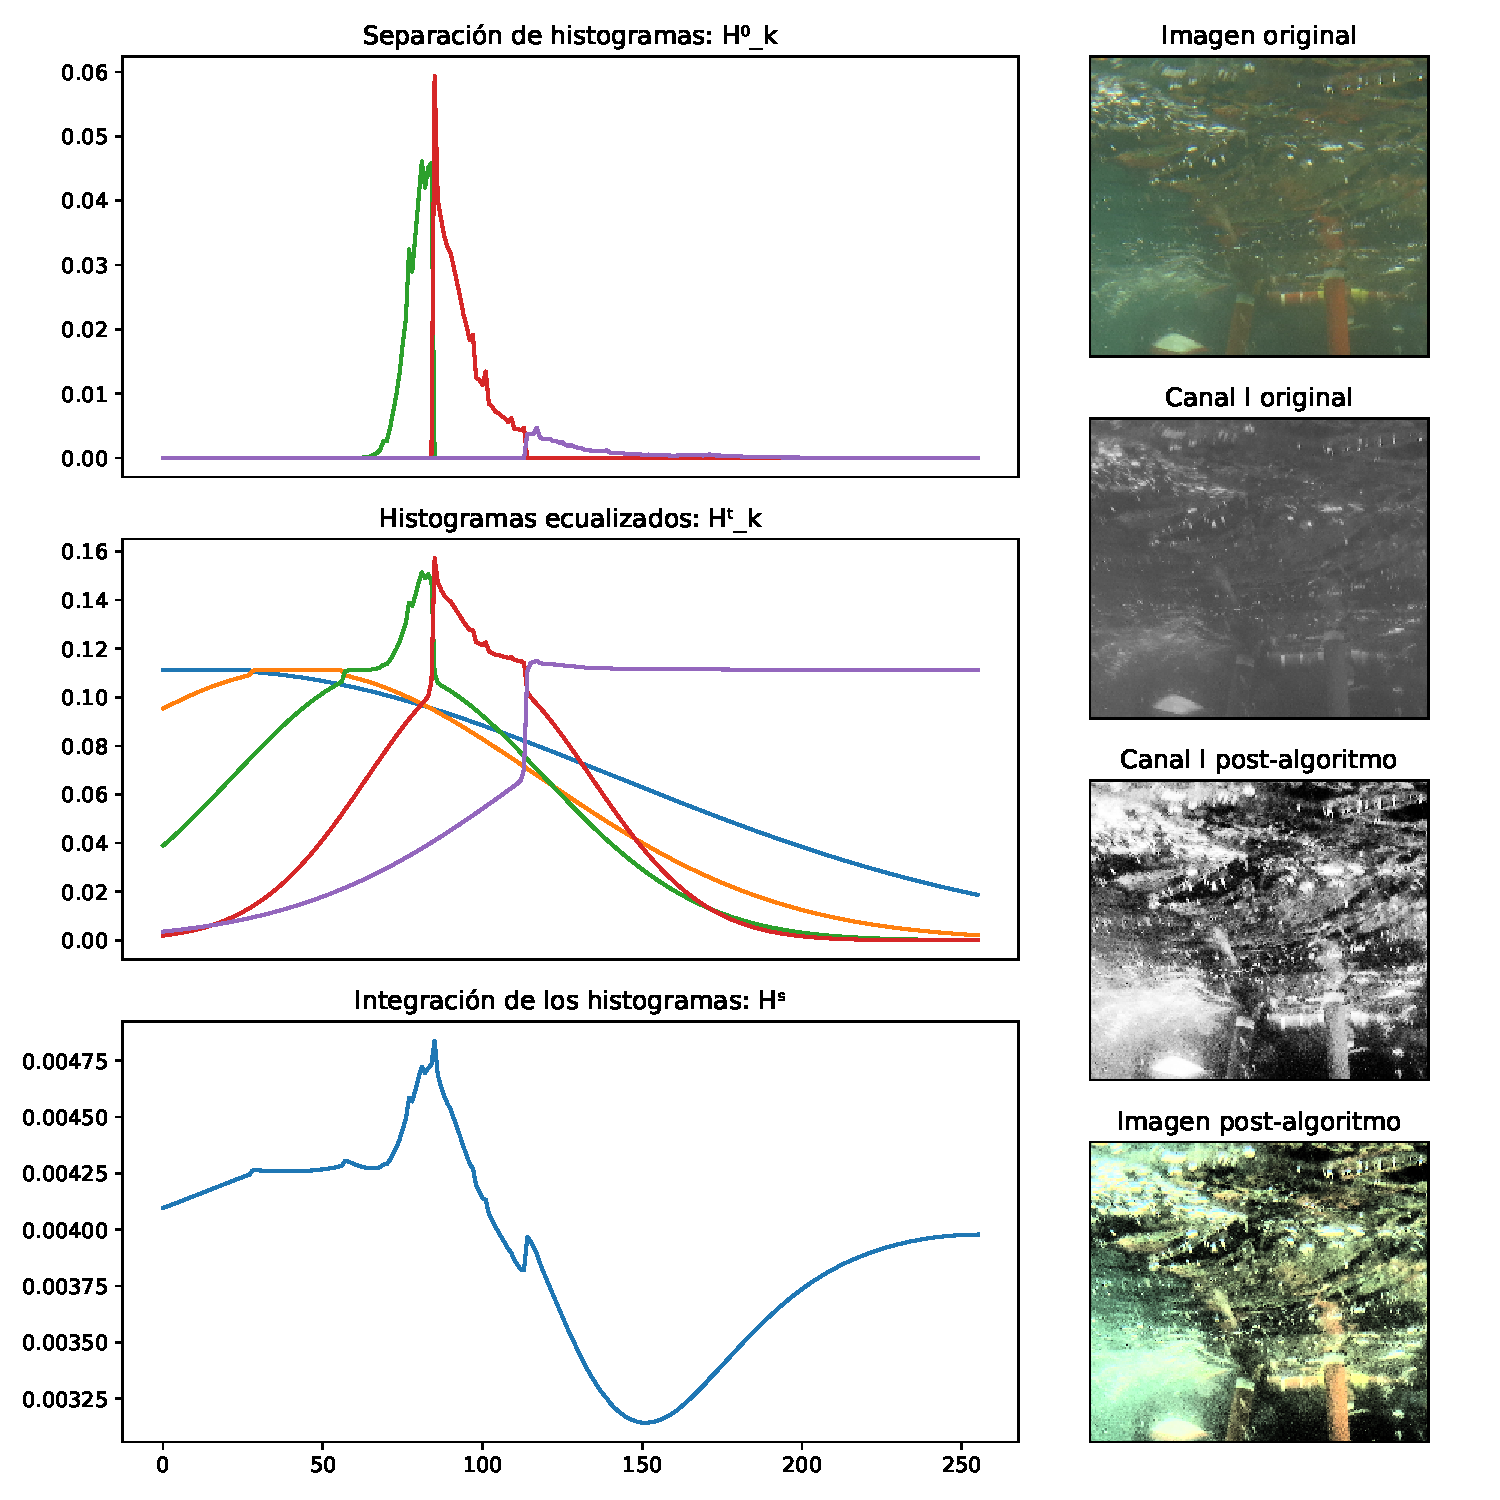
\includegraphics[height=9cm]{imgs/1908iv-11115.pdf}
  \caption{\texttt{[1, 1, 1, 1, 5]}}
\end{minipage}%
\end{figure}

\subsection{Ejemplo 3}
Usamos la imagen \texttt{backlight-la-nacion}, con parámetros $\alpha = 0.5$, $\beta = 0.4$, $\gamma = 0.1$.

\begin{figure}[H]
\begin{minipage}[c]{0.48\linewidth}
  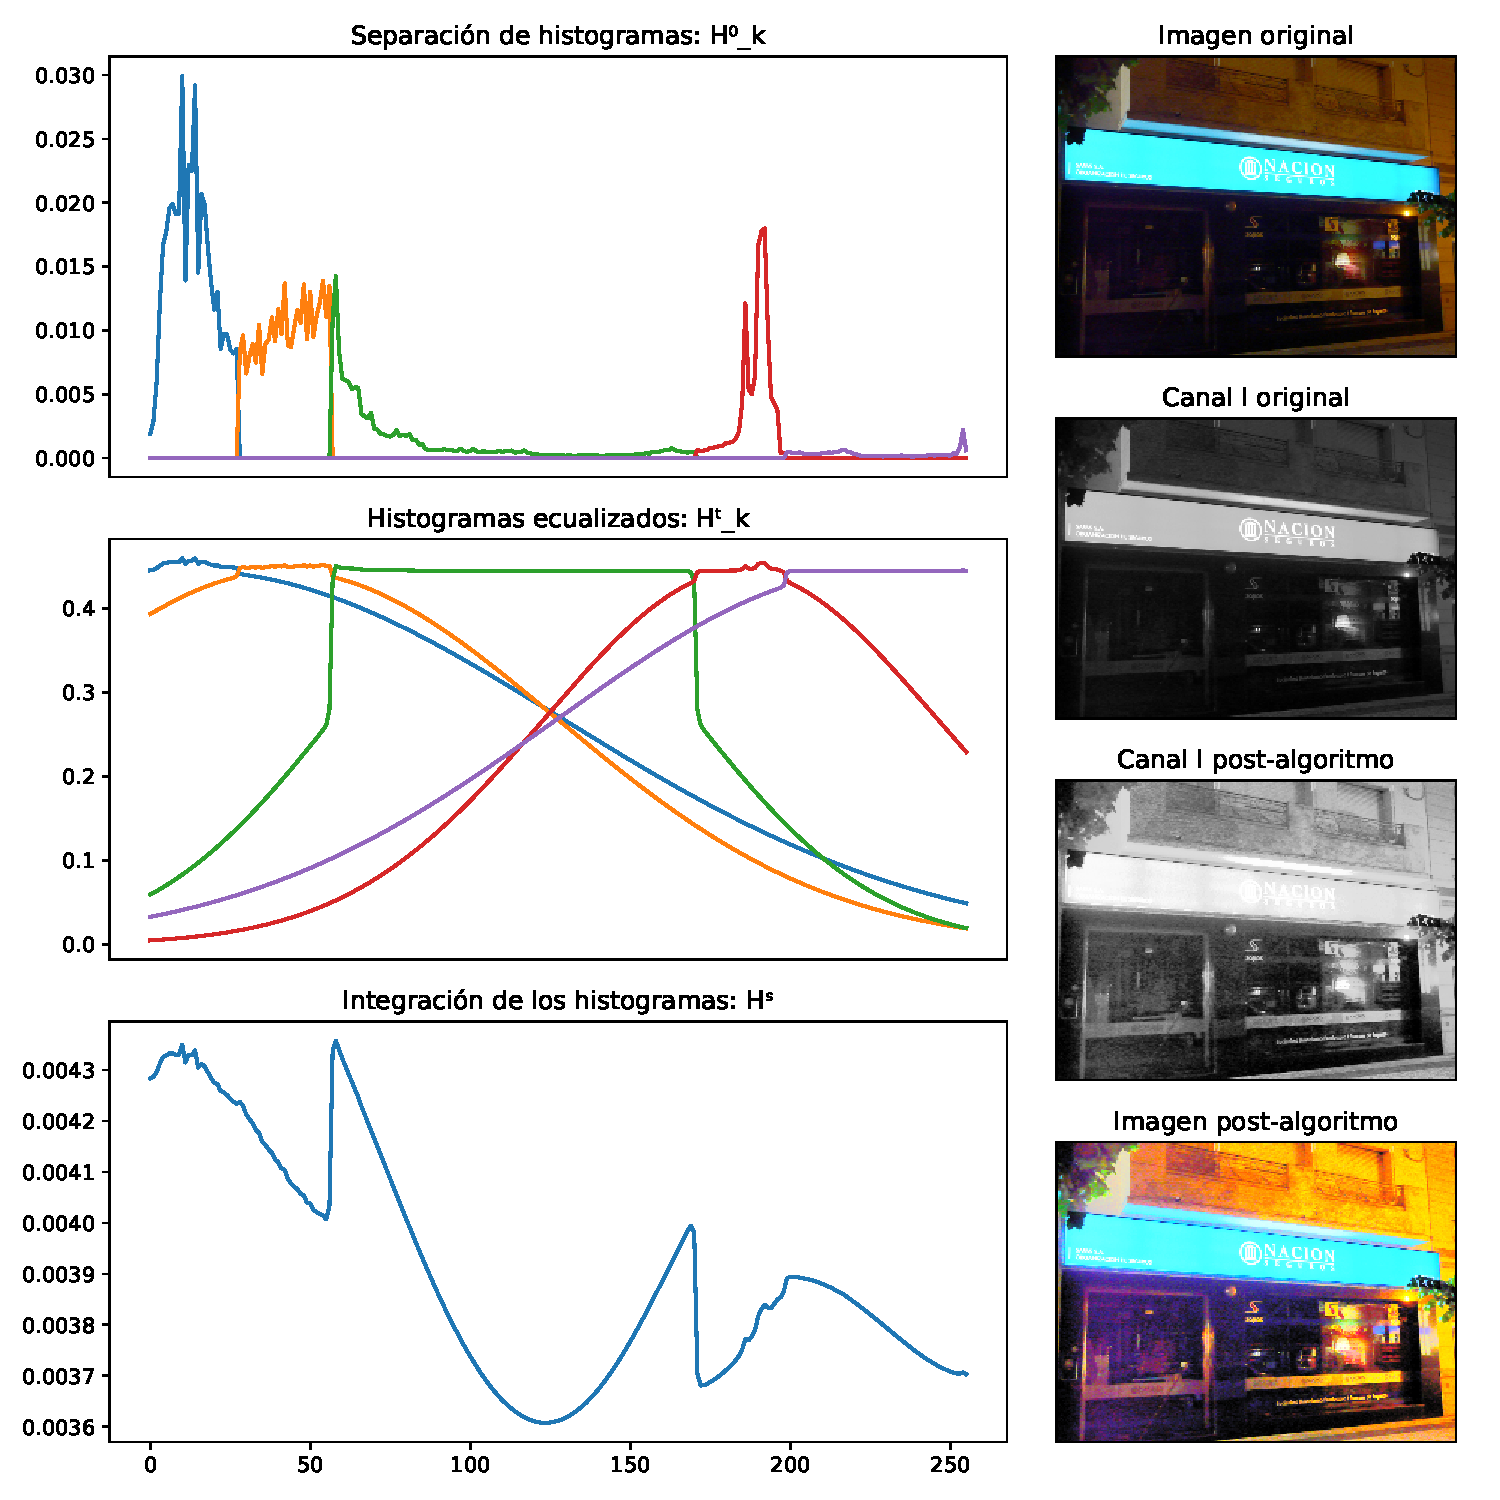
\includegraphics[height=9cm]{imgs/backlightnacion-11412.pdf}
  \caption{\texttt{[1, 1, 4, 1, 2]}}
\end{minipage}
\hfill
\begin{minipage}[c]{0.48\linewidth}
  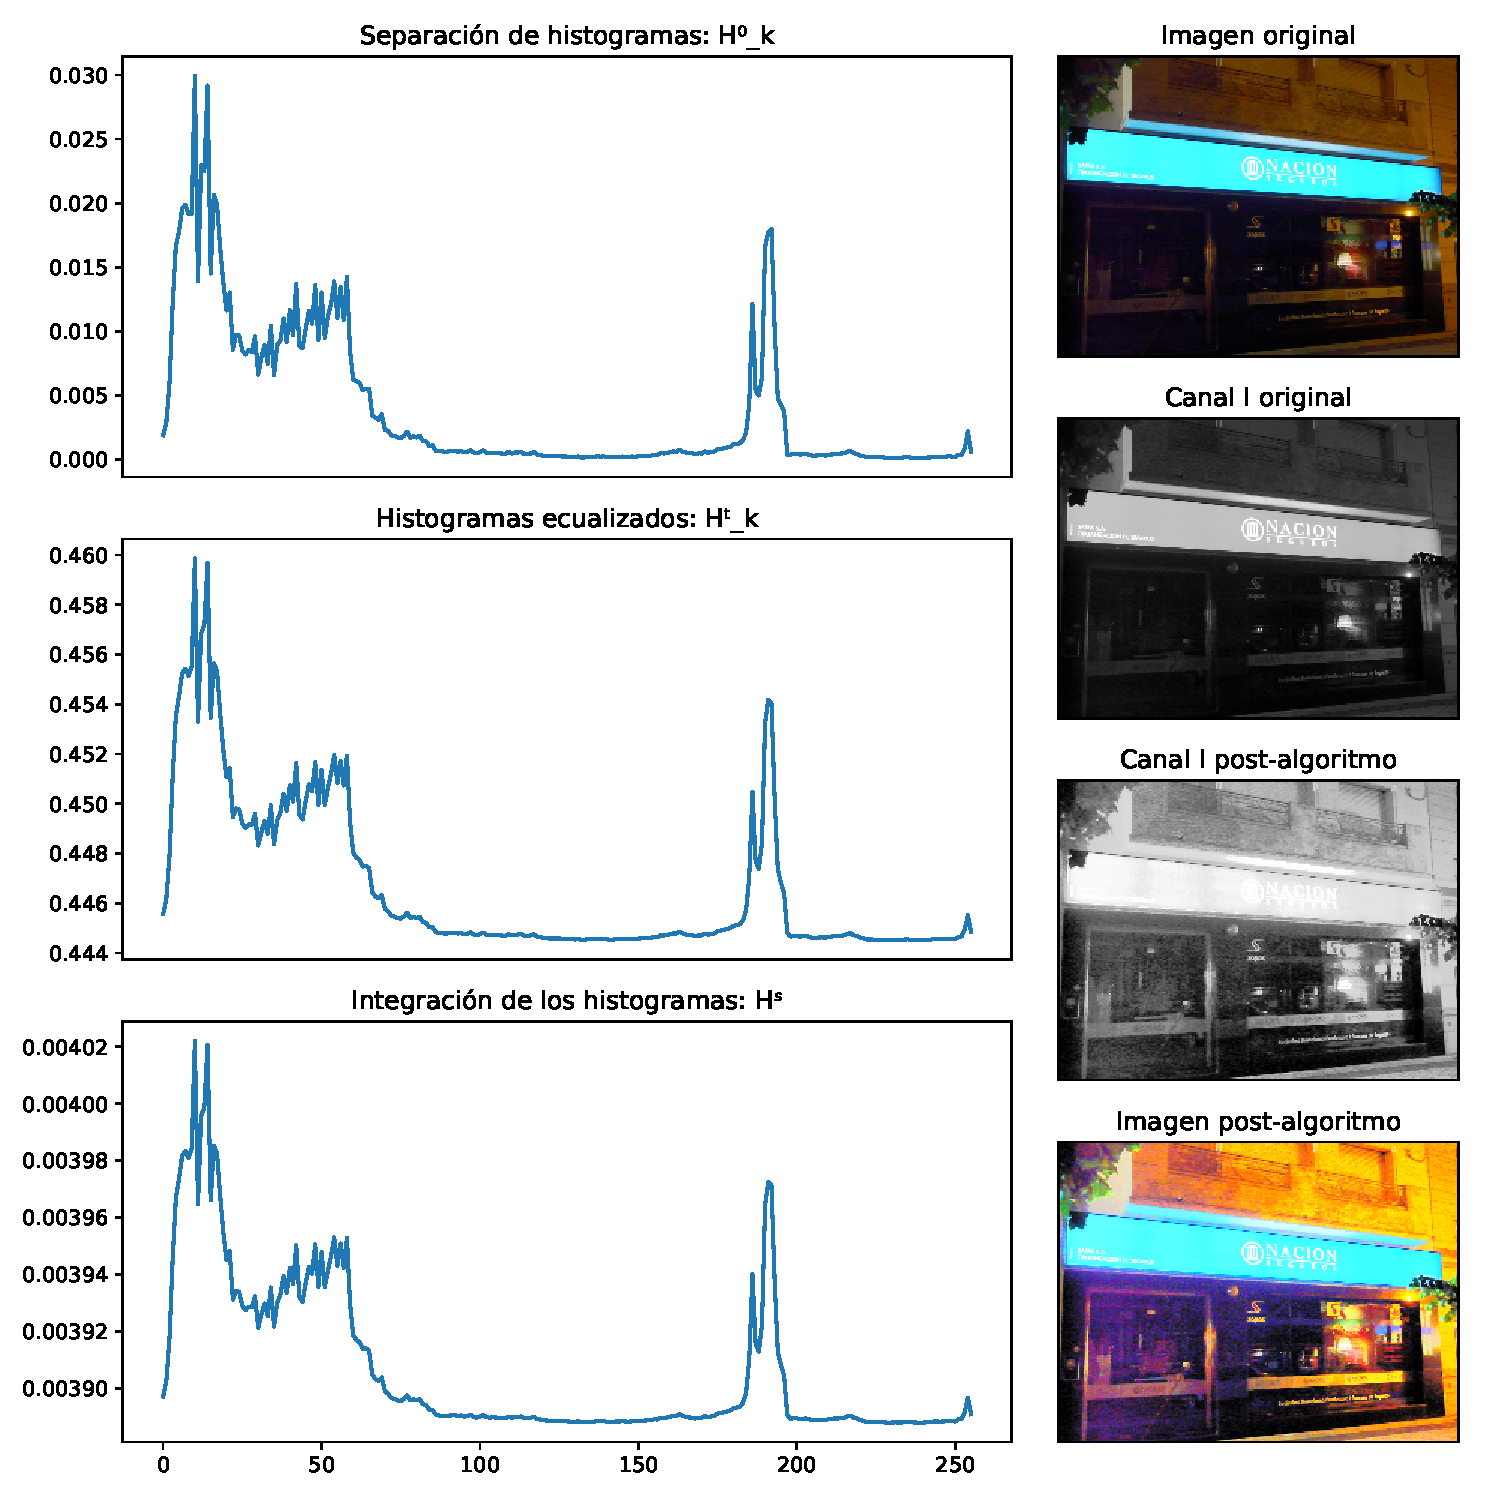
\includegraphics[height=9cm]{imgs/backlightnacion-1.pdf}
  \caption{\texttt{[1]}}
\end{minipage}%
\end{figure}

\begin{figure}[H]
\begin{minipage}[c]{0.48\linewidth}
  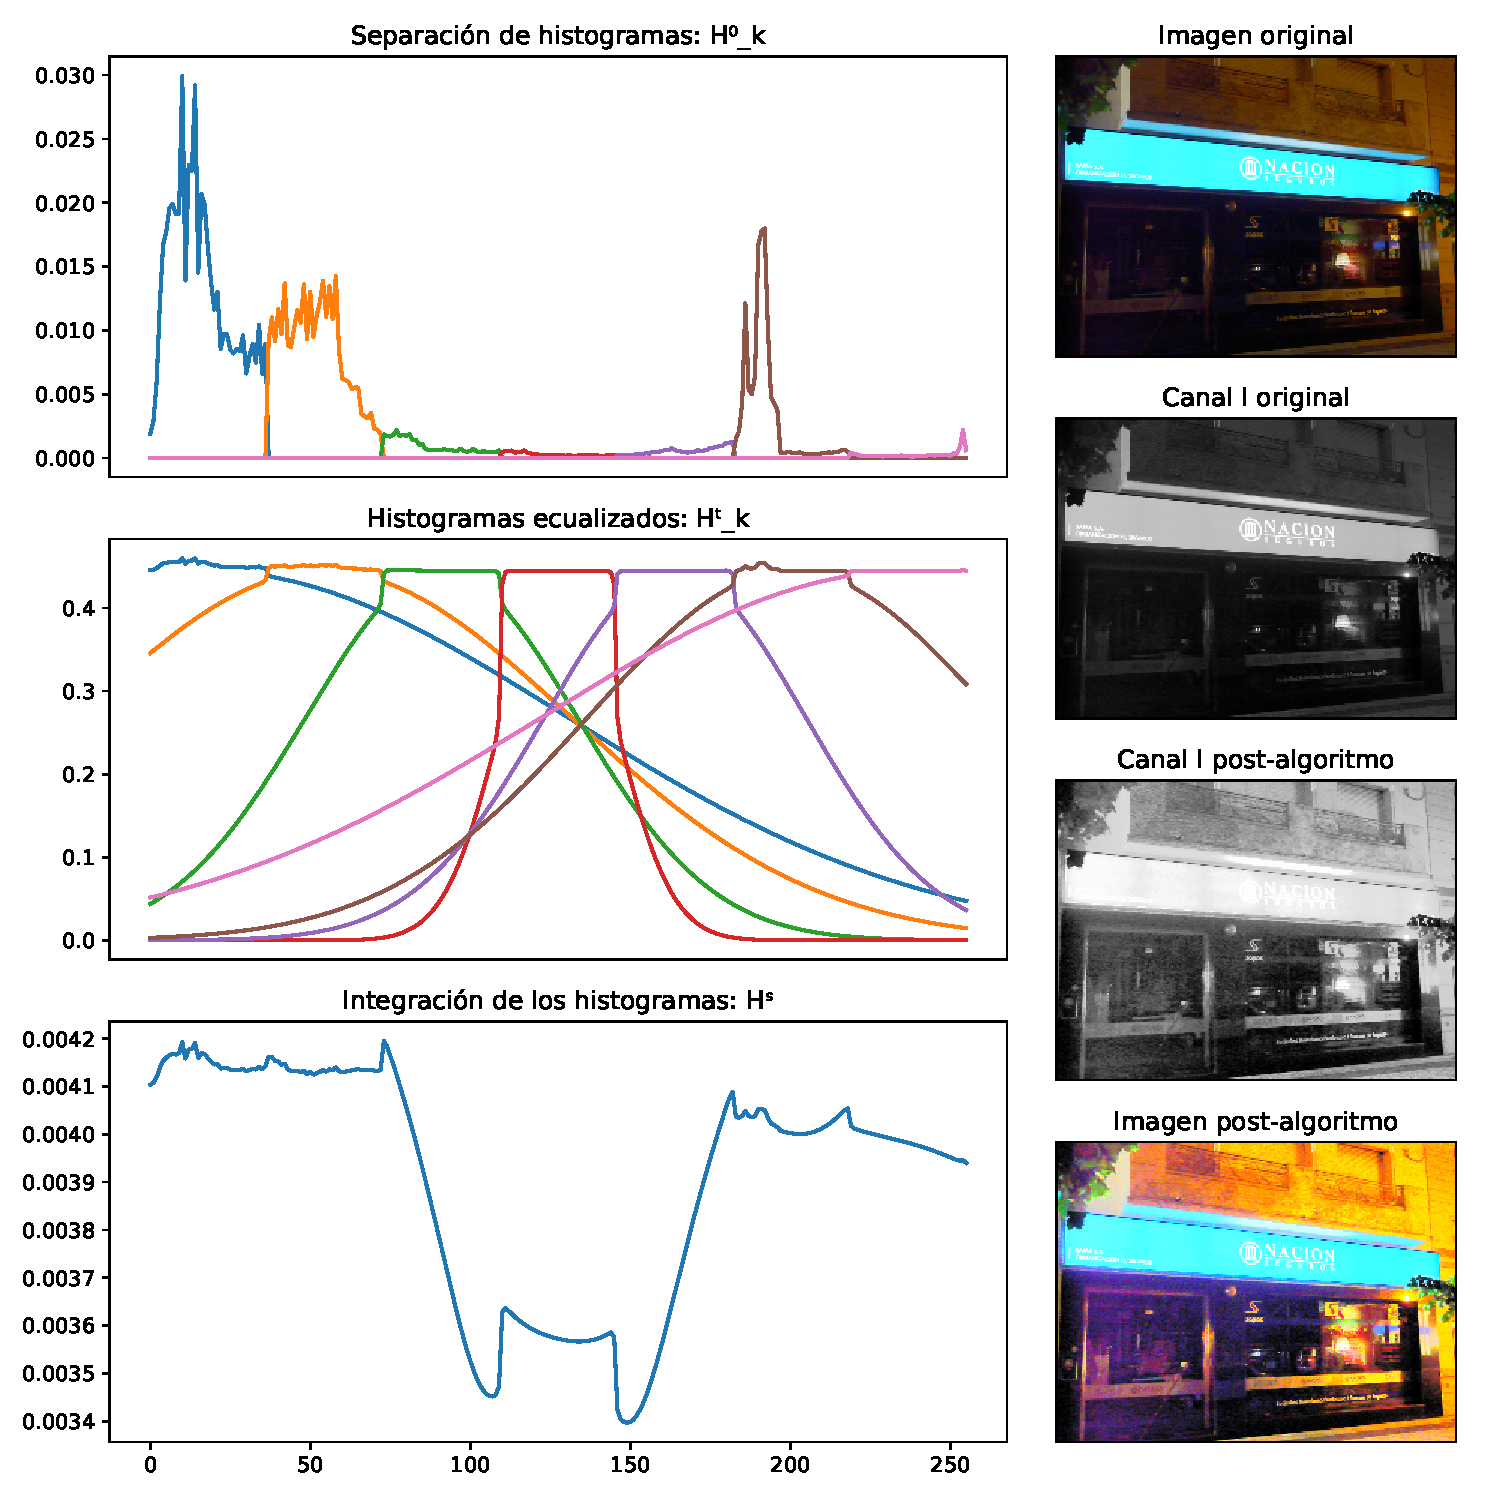
\includegraphics[height=9cm]{imgs/backlightnacion-1111111.pdf}
  \caption{\texttt{[1, 1, 4, 1, 2]}}
\end{minipage}
\hfill
\begin{minipage}[c]{0.48\linewidth}
  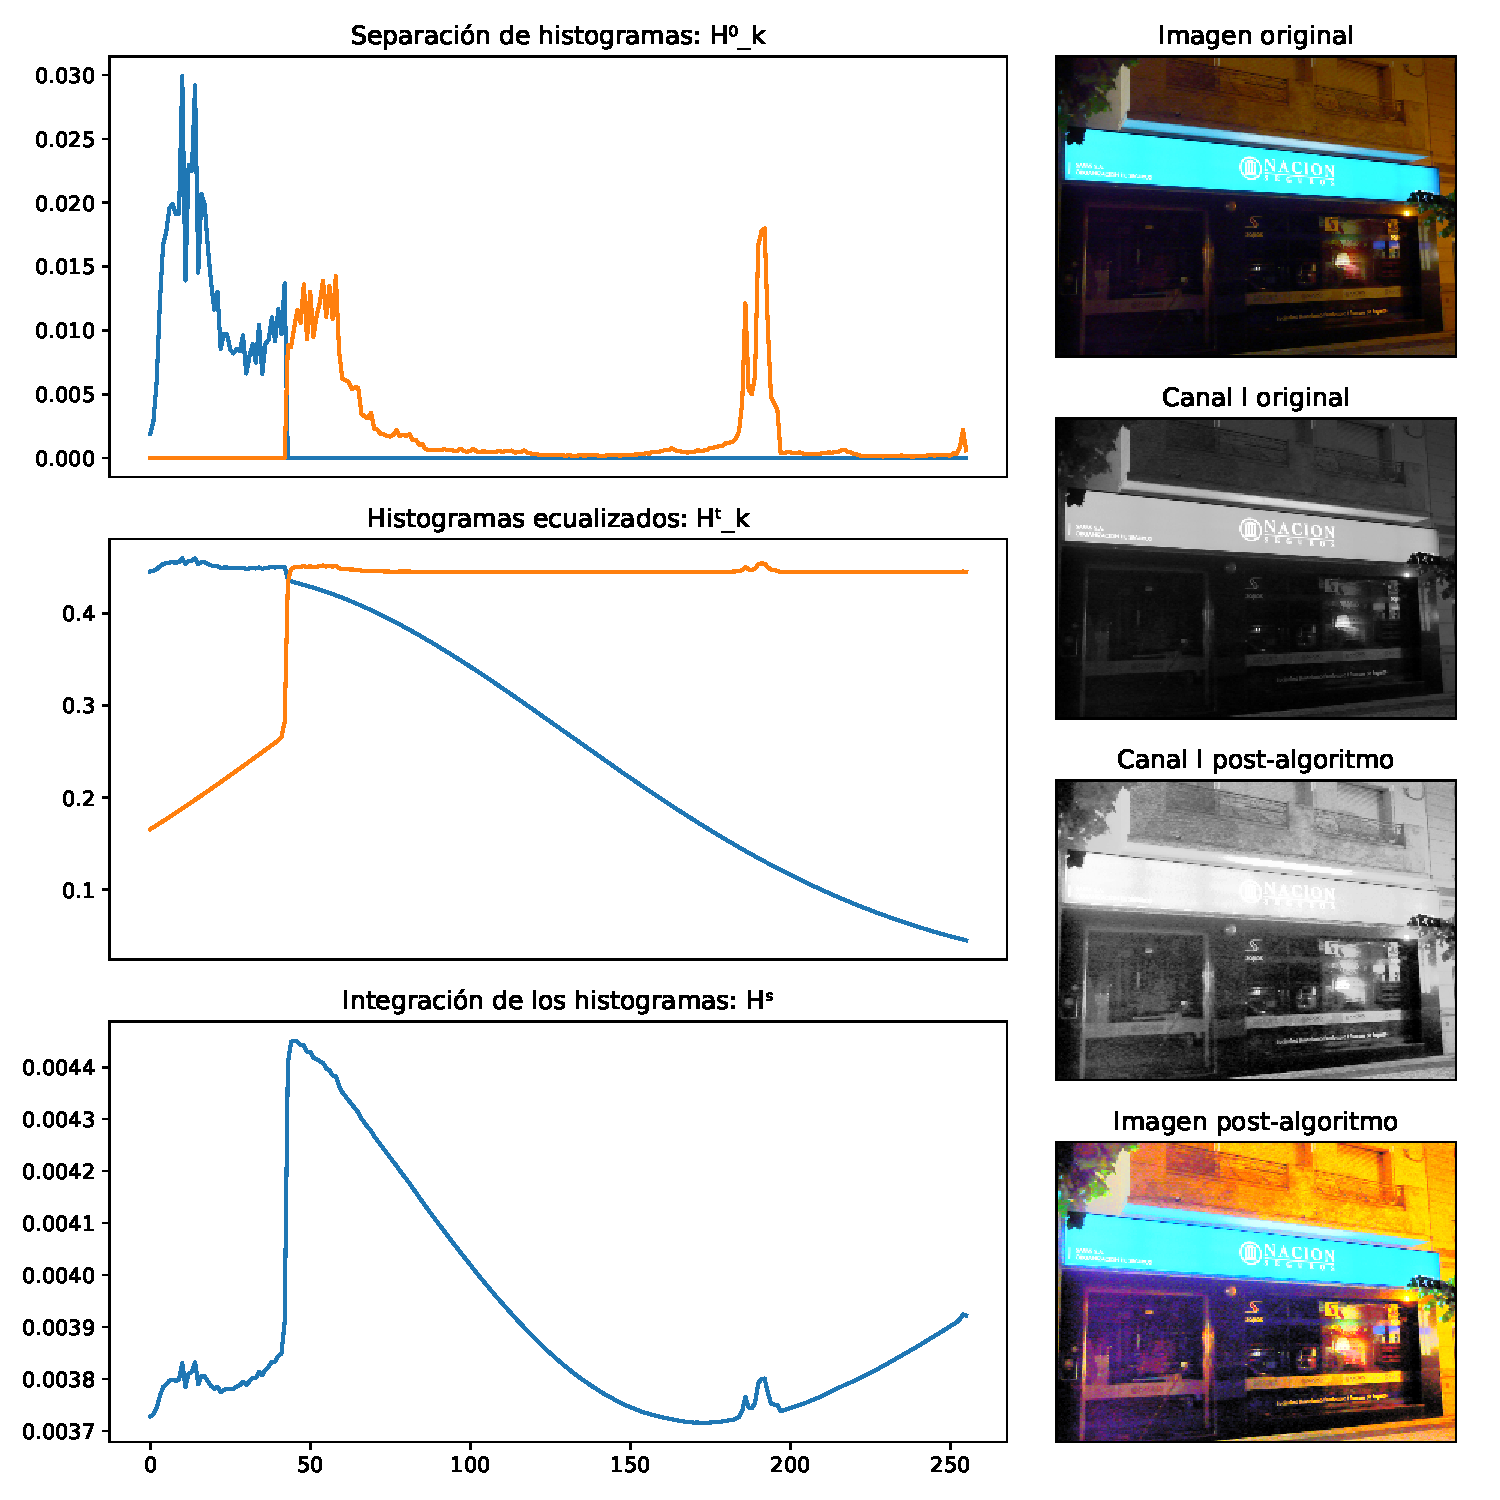
\includegraphics[height=9cm]{imgs/backlightnacion-15.pdf}
  \caption{\texttt{[1]}}
\end{minipage}%
\end{figure}
